\chapter{Introducción} % (fold)
\label{cha:introduccion}

\section{Motivación} % (fold)
\label{sec:motivacion}

Este proyecto surgió de la problemática de algunos trabajos realizados dentro del Laboratorio de Arquitectura de Computadoras que compartían las mismas necesidades: la obtener y convertir señales de sensores, contar eventos de sistemas digitales por hardware, y que transmitir los datos obtenidos por un canal unico de comunicacion serial. \\

Motivaciones: 

\begin{itemize}
	\item Económicas:
	    \begin{itemize}
	        \item Materiales a nuestro alcance.
	        \item Posibilidad de realizar un producto viable.
	    \end{itemize}
	\item Académicas:
	    \begin{itemize}
	        \item Oportunidad de mejorar y facilitar las mediciones de sensores analógicos y recolectar datos de señales digitales para los alumnos que realicen proyectos en el LAC (Laboratorio de Arquitectura de Computadoras). Logrando asi un concentrador generico adaptable y multiplataforma
	    \end{itemize}
	\item De Investigación:
	    \begin{itemize}
	        \item Investigar como acelerar los procesos de desarrollo de software y hardware.
	        \item Poner en uso una metodología ágil en el software.
	        \item Poner en uso una metodología ágil en el hardware.
	    \end{itemize}
	\item De Extensión:
	    \begin{itemize}
	        \item Laboratorios de Universidades de la RUNIC.
	        \item Empresas del medio.
	    \end{itemize}
	\item Tecnológicas:
	    \begin{itemize}
	        \item Utilizar tecnología madura.
	        \item Utilizar tecnología bien documentada.
	        \item Utilizas SysUML para documentar nuestro sistema
	        \item Utilizar tecnología muy difundida.
	    \end{itemize}
\end{itemize}

% section motivacion (end)

\section{Objetivos} % (fold)
\label{sec:objetivos}

\subsection{Objetivo principal} % (fold)
\label{sec:objetivo_principal}

Diseño y construcción de una placa de instrumentación de señales digitales y analógicas autónoma con un sistema de comunicación.

% section objetivos_principales (end)

\subsection{Objetivos Secundarios a Alcanzar en el Tiempo Estimado} % (fold)
\label{sec: objetivos_secundarios}

\begin{itemize}
	\item La placa debe leer entre 8 y 16 señales analógicas.
    \item La placa debe contar eventos digitales con 2 o 3 contadores distintos.
    \item La placa debe transmitir los datos digitales a través de un protocolo serial, a alguna otra placa de desarrollo o procesador.
    \item El sistema debe tener un control de ganancias programable.
    \item Lograr que el sistema tenga menor a 1,2 Vatios.
    \item Lograr que el sistema tenga la mejor inmunidad al ruido.
    \item El sistema debe ser lo mas pequeño posible.
    \item Se debe tener una sensibilidad apta para poder medir un sensor de campo electrostático.
    \item Se debe controlar el arranque y velocidad de un motor brushless con un PWM (pulse-width modulation).
    \item El sensor de campo electrostático debe tener una placa por separado para el manejo de la potencia.
    \item Se debe desarrollar un servidor web en alguna placa de desarrollo para poder controlar todas las acciones del sensor remotamente.
    \item El servidor web debe poder guardar datos de las lecturas que se realizan del sensor en una base de datos (preferentemente MySQL).
    \item Escribir la documentación sobre las instrucciones de uso para manejar el software embebido en la placa.
    \item Realizar una prueba de campo.
\end{itemize}
% section objetivos_secundarios (end)

\section{Herramientas de modelado} % (fold)
\label{sec:herramientas_de_modelado}

Para facilitar la documentación, decidimos utilizar SysUML para documentar nuestro sistema. Para esto, utilizamos la herramienta Enterprise Architect, que nos permite partir de un modelo base y reutilizar los componentes en todos los diagramas, generando vínculos que facilitan el entendimiento general del sistema. 

% section herramientas_de_modelado (end)

\section{Requerimientos} % (fold)
\label{sec:requerimientos}

\subsection{Requerimientos funcionales} % (fold)
\label{sub:requerimientos_funcionales}

Partiendo de los objetivos planteados, podemos formalizar una lista de requerimientos para nuestro sistema.

\begin{itemize}
	\item Se deberían poder recibir datos de hasta 8 sensores analógicos en modo singular o equilibrado [1.1]
	\item Se debería poder configurar, mediante una interfaz de usuario, cada canal analógico por separado para medir en modo diferencial, modo canal único, o no medir. [1.2]
	\item Se deberían poder contar eventos de hasta 4 señales externas. [1.3]
	\item Se debería poder configurar una ganancia especifica para el conversor analógico digital mediante una interfaz de usuario. [1.4]
	\item Se debería poder configurar un tiempo entre mediciones especifico para cada entrada mediante una interfaz de usuario. [1.5]
	\item El canal de comunicación entre la plataforma y el sistema embebido o controlador debería ser serial. [1.6]
	\item La plataforma debería poder controlar y obtener mediciones del sensor de campo electrostático [1.7]
	\item Se debería diseñar un caso de uso de sistema embebido que trabaje junto con la plataforma. [1.8]
\end{itemize}

% subsection requerimientos_funcionales (end)

\subsection{Requerimientos no funcionales} % (fold)
\label{sub:requerimientos_no_funcionales}

\begin{itemize}
    \item El sistema debería consumir lo menos posible. [2.1]
    \item El sistema debería tener la mayor inmunidad al ruido posible [2.2]
	\item La plataforma de instrumentación debería ser portable, es decir, debería permitir que la cantidad de sistemas embebidos compatibles sea lo mayor posible. [2.3]
\end{itemize}

% subsection requerimientos_no_funcionales (end)

% section requerimientos (end)

\section{Características generales} % (fold)
\label{sec:caracteristicas_generales}

En una primera aproximación del sistema a construir, se puede establecer que se trata de un sistema capaz de recibir señales de distintos sensores digitales y analógicos. En caso que sean analógicos, convertir las señales a digital usando un conversor A-D de alta ganancia, que permita tanto entradas en modo único como como diferencial. Luego de ser convertidas, estas señales deben ser enviadas mediante un protocolo de comunicación a otro sistema que realice las acciones que deba realizar en función de los datos enviados.

En nuestro contexto interactúan 3 actores: Un usuario, uno o más sensores, y un controlador que por el momento no hacemos mención de sus características, por lo que lo llamamos simplemente ``controlador''.

\begin{figure}[h]
  \centering
  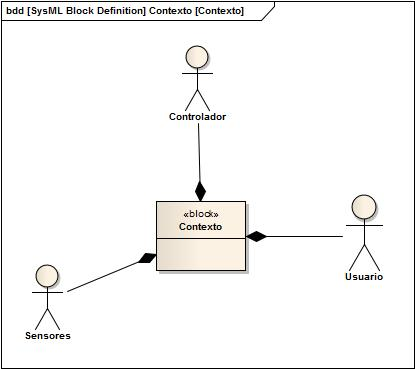
\includegraphics[width=0.80\textwidth, height = 9cm]{contexto1}
  \caption{Contexto del sistema}\label{fig:contexto1}
\end{figure}

% section caracteristicas_generales (end)

\section{Método de desarrollo} % (fold)
\label{sec:metodo_de_desarrollo}

El método de desarrollo utilizado es el desarrollo iterativo con entrega incremental. Este modelo se ilustra en la Figura \ref{fig:MetodoDeDesarrollo}. En esta metodología de desarrollo el trabajo se divide en iteraciones en las cuales el producto va evolucionando. 
Un aspecto fundamental para guiar el desarrollo incremental es priorizar los requerimientos y los objetivos en función del valor que aportan al cliente. De esta manera se van añadiendo nuevos requerimientos o mejorando los que ya se completaron. Al finalizar cada iteración se obtiene un prototipo funcional.

\begin{figure}[h]
  \centering
  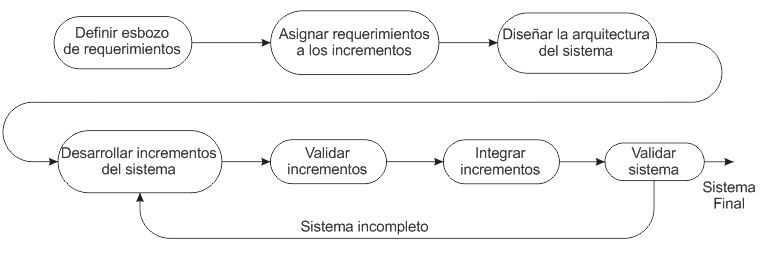
\includegraphics[width=0.80\textwidth, height = 4cm]{MetodoDeDesarrollo}
  \caption{Desarrollo incremental}\label{fig:MetodoDeDesarrollo}
\end{figure}

% section metodo_de_desarrollo (end)

\section{Casos de uso} % (fold)
\label{sec:casos_de_uso}

Dado el contexto, el sistema se puede describir de una manera general mediante un diagrama de caso de uso. El diagrama puede verse en la Figura \ref{fig:casouso1}. En esta Figura, se puede ver plasmados los requerimientos.

\begin{figure}[h]
  \centering
  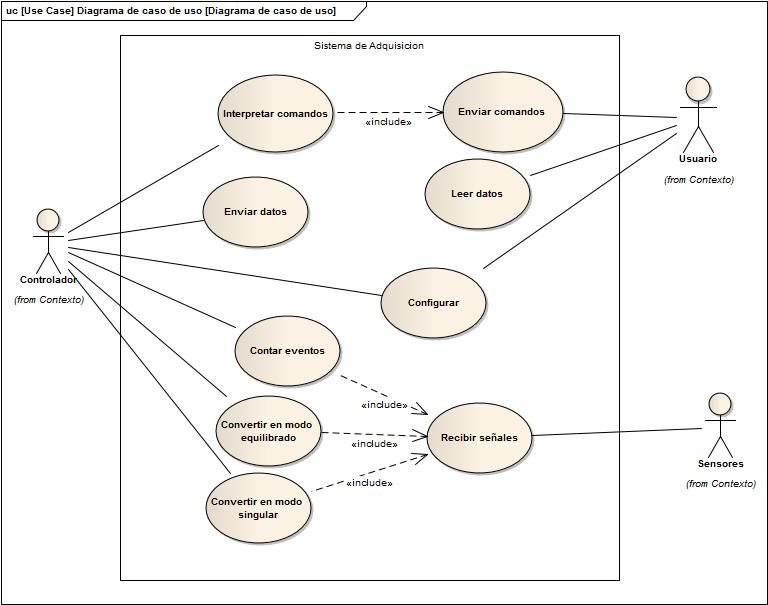
\includegraphics[width=0.80\textwidth, height = 11cm]{casouso1}
  \caption{Diagrama de caso de uso del sistema de adquisición}\label{fig:casouso1}
\end{figure}

El caso de uso ``configurar'' esta generalizado. Las acciones que incluye este caso son:
\begin{itemize}
	\item Configurar la interfaz serial
	\item Configurar canal en modo singular
	\item Configurar canal en modo equilibrado
	\item Configurar contador de eventos
	\item Configurar ganancia del del conversor
	\item Configurar intervalo de medicion para conversion analogica
\end{itemize}

% section casos_de_uso (end)

% chapter introduccion (end)